\documentclass[12pt]{article}
\usepackage{sbc-template}
\usepackage{amsmath,amssymb}
\usepackage{graphicx,url,booktabs}
\usepackage[utf8]{inputenc}
\usepackage[english]{babel}
\usepackage{enumitem}
\usepackage{pifont}
\usepackage{array}
\usepackage{xcolor}
\usepackage{breakcites}
\graphicspath{{figures/}}
\usepackage{caption}
\captionsetup[figure]{font={small,bf},skip=3pt}
\captionsetup[table]{font={footnotesize,bf}}
\setlength{\textfloatsep}{5pt plus 2pt minus 2pt}
\setlength{\intextsep}{5pt plus 2pt minus 2pt}
\setlength{\floatsep}{5pt plus 2pt minus 2pt}
\newcommand{\cmark}{\textcolor{green!60!black}{\ding{51}}}
\newcommand{\xmark}{\textcolor{red!70!black}{\ding{55}}}
\usepackage[hidelinks,colorlinks=true,allcolors=black]{hyperref}

% patch p/ o bug \bbl@normalsf (sbc-template + babel em TeXLive recente)
\makeatletter
\gdef\normalsfcodes{}
\gdef\bbl@normalsf{}
\AddToHook{begindocument/before}[patch.normalsfcodes]{%
  \gdef\normalsfcodes{}%
  \gdef\bbl@normalsf{}%
}
\DeclareHookRule{begindocument/before}{patch.normalsfcodes}{before}{babel}
\AddToHook{shipout/before}{\gdef\normalsfcodes{}\gdef\bbl@normalsf{}}
\makeatother

% ============================================================
% RASCUNHO: artigo CURTO (SBSeg, ~6 paginas). Numeros marcados
% PROVISORIO sao do scan parcial (atualizar ao fechar o censo).
% Intro/Relacionados: preencher apos ler os PDFs completos (sem plagio).
% ============================================================

\title{How Secure Is Your Base? A Recent Multi-Scanner\\
Census of Linux Operating-System Images on Docker Hub}

\author{Anonymous}
\address{Anonymous Institution}

\begin{document}
\maketitle

\begin{abstract}
% PROVISORIO: fechar com numeros finais do censo
Every container starts from an operating-system (OS) base image, yet the
security posture of these foundational images is usually measured with a
single scanner and on samples that age quickly. We present a recent,
multi-scanner census of the OS base images on Docker Hub: the
\textbf{5{,}606} unique \texttt{amd64} images across the \textbf{21}
repositories of Docker Hub's \emph{Operating systems} category, each scanned by
\textbf{13} independent open-source scanners spanning vulnerabilities, SBOM,
misconfiguration, secrets and malware. % TODO numeros finais
We find that (i)~vulnerability posture varies sharply by distribution, with
the RHEL family carrying the most critical/high findings and Alpine the
fewest; (ii)~image staleness is a strong predictor of vulnerability count,
which grows monotonically with time-since-rebuild; (iii)~the four
package-vulnerability engines barely agree (pairwise Jaccard $\le 0.31$), with
OSV-Scanner and Clair nearly disjoint from the rest; and (iv)~about one in
five historically-published OS images can no longer be pulled by a modern
Docker because they use a legacy manifest schema. We release the pipeline and
the consolidated multi-scanner dataset, to our knowledge the first
OS-base-focused one, on acceptance.
\end{abstract}

% ============================================================
\section{Introduction}
\label{sec:intro}
Containers are now a default unit of software delivery: Docker reports more
than 20~million developers using its tools and, in its 2025 survey, 92\% of IT
professionals using containers~\cite{docker2025stateofappdev}, while the Cloud
Native Computing Foundation finds most organisations running the majority of
their applications in containers~\cite{cncf2024survey}. Underneath them sits
Docker Hub, the largest public registry, with on the order of 8.3~million
image repositories and hundreds of billions of cumulative
pulls~\cite{dockerindex2024}. Every one of those images ultimately begins with
a single line, \texttt{FROM} an operating-system (OS) base image, and a
handful of bases are the common root of nearly all of them: \texttt{alpine},
\texttt{ubuntu}, \texttt{debian} and \texttt{busybox} each record more than a
billion pulls, and Debian, Alpine and Ubuntu dominate the base-image choice of
the ecosystem~\cite{anchore2024osbreakdown}. Because a flaw in a base image is
inherited, unchanged, by every image built on it~\cite{shu2017dockerhub}, the
security posture of these few OS bases is a property the whole ecosystem
inherits.

That inherited posture is poor and consequential. Software-supply-chain
attacks are projected to cost USD~60~billion in
2025~\cite{cybersecurityventures2023supplychain} and Gartner predicted that
45\% of organisations would suffer such an attack by
2025~\cite{gartner2021supplychain}; meanwhile popular Docker Hub images carry
hundreds of known vulnerabilities on average, many of them years
old~\cite{netrise2024}, against a backdrop of record CVE disclosure
(46{,}407 CVEs in 2025, about 127 per day)~\cite{nvd2025growth}. Worse, some of
the most-pulled OS bases are no longer maintained (every official
\texttt{centos} tag reached end-of-life in June~2024) yet remain in heavy
use.

Despite this central role, the security posture of OS base images is usually
measured with a \emph{single} scanner and on samples that age quickly. The
large-scale Docker Hub measurements rely on one detector each~\cite{shu2017dockerhub,zerouali2019outdated,liu2020understanding,shi2025drdocker},
and the studies that \emph{do} compare scanners run on small, controlled
samples (44 and 380 images)~\cite{kaur2021scientific,mills2023longitudinal}.
No recent work measures the OS base images specifically, with a heterogeneous
multi-scanner battery, as a current census. This paper fills that gap.

\paragraph{Contributions.}
\begin{itemize}[leftmargin=1.4em,itemsep=1pt,topsep=2pt]
\item A \textbf{recent multi-scanner census} of OS base images on Docker Hub:
13 scanners over 5{,}606 unique \texttt{amd64} images of the 21
\emph{Operating systems} repositories (Section~\ref{sec:method}).
\item A \textbf{per-distribution security posture} and a measured
\textbf{staleness-vulnerability} relationship (Sections~\ref{sec:rq1},~\ref{sec:rq2}).
\item A \textbf{four-engine divergence} measurement on the OS-package layer,
including Clair, showing the chosen scanner dominates the reported posture
(Section~\ref{sec:rq3}).
\item A supply-chain \textbf{longevity finding}: a large share of
historically-pulled OS images are no longer installable by a modern Docker
(legacy manifest schema), and end-of-life bases remain heavily pulled.
\item \textbf{A released artifact and dataset.} We release the scan pipeline
and the consolidated multi-scanner dataset, the per-image reports of all 13
scanners over the OS census; to our knowledge it is the first OS-base-focused
multi-scanner dataset, letting the measurement be audited, reproduced and
extended (released on acceptance).
\end{itemize}

% ============================================================
\section{Related Work}
\label{sec:related}
\paragraph{Large-scale Docker Hub and base-image measurements.}
The security of Docker Hub has been measured at scale since Shu et
al.~\cite{shu2017dockerhub}, who scanned 356{,}218 images with a single
detector and documented that a flaw in a base image propagates to every image
built on it. Subsequent measurements kept the single-detector design: Liu et
al.~\cite{liu2020understanding} reached 2.2~million images, Zerouali et
al.~\cite{zerouali2019outdated} measured \emph{technical lag} in 7{,}380
Debian-based images and found no release free of vulnerabilities, Wist et
al.~\cite{wist2021vulnerability} analysed 2{,}500 images, and the recent
Dr.~Docker~\cite{shi2025drdocker} ranked 33{,}952 influential images by pull
count yet sub-sampled only 3{,}000 for vulnerabilities with one engine.
Closest to our subject, Haque and Babar~\cite{haque2022wellbegun} studied the
exploitability and impact of vulnerabilities across 261 official base images
and reported a counter-intuitive result we revisit in Section~\ref{sec:rq5}:
highly-exploitable vulnerabilities are \emph{more} frequent in minimal images
such as Alpine and BusyBox, while large distributions carry the higher-impact
ones. Every one of these studies relies on a single vulnerability scanner, so
its reported posture inherits that tool's blind spots.

\paragraph{Inter-scanner divergence.}
A second line shows that a scan result depends heavily on the scanner. Imtiaz
et al.~\cite{imtiaz2021comparative} run nine software-composition-analysis
tools over the same projects and observe counts spanning an order of
magnitude; Javed and Toor~\cite{javed2021evaluation,javed2021quality} report
that container scanners miss a large fraction of vulnerabilities. On containers
the side-by-side comparisons have been small: Kaur et
al.~\cite{kaur2021scientific} use four scanners over 44 images and Mills et
al.~\cite{mills2023longitudinal} six over 380. The closest and most recent,
Churakova et al.~\cite{churakova2026vex}, evaluate seven scanner and VEX tools
on 48 images and find counts ranging from 191 to 18{,}680, with the
best-agreeing pair (Trivy and Grype) overlapping on only about 69\%. We measure
the same divergence at two orders of magnitude more images, restricted to the
OS-base subset, including Clair, and crossed with image age and distribution.

\paragraph{Gap.}
No recent study measures the operating-system base images of Docker Hub
specifically, with a heterogeneous multi-scanner battery, as a current census;
and the prevalence and popularity of \emph{end-of-life} OS images that remain
in heavy use has, to our knowledge, not been measured. We address both.

\begin{table}[!htbp]
\centering
\caption{Positioning against prior OS/base-image measurements.}
\label{tab:related}
\renewcommand{\arraystretch}{1.2}
\footnotesize
\begin{tabular}{l c r c c c}
\toprule
\textbf{Work} & \textbf{Year} & \textbf{Images} & \textbf{Scanners} & \textbf{OS-focused} & \textbf{Cross-scanner} \\
\midrule
Shu et al.~\cite{shu2017dockerhub}        & 2017 & 356{,}218 & 1 & \xmark & \xmark \\
Zerouali et al.~\cite{zerouali2019outdated} & 2019 & 7{,}380 & 1 & \cmark{}\,(Debian) & \xmark \\
Kaur et al.~\cite{kaur2021scientific}     & 2021 & 44 & 4 & \xmark & \cmark \\
Mills et al.~\cite{mills2023longitudinal} & 2023 & 380 & 6 & \xmark & \cmark \\
Haque \& Babar~\cite{haque2022wellbegun} & 2022 & 261 & 1 & \cmark & \xmark \\
Shi et al.\ (Dr.\ Docker)~\cite{shi2025drdocker} & 2025 & 33{,}952 & 1 & \xmark & \xmark \\
Churakova et al.~\cite{churakova2026vex} & 2026 & 48 & 7 & \xmark & \cmark \\
\midrule
\textbf{This work} & \textbf{2026} & \textbf{5{,}606} & \textbf{13} & \cmark & \cmark \\
\bottomrule
\end{tabular}
\end{table}

% ============================================================
\section{Methodology}
\label{sec:method}
% Esta secao e NOSSA, escrita original.

\paragraph{Corpus.}
We take as our corpus the operating-system base images that Docker Hub itself
lists under its \emph{Operating systems} category: 22 repositories (e.g.\
\texttt{alpine}, \texttt{ubuntu}, \texttt{debian}, \texttt{centos},
\texttt{busybox}, \texttt{amazonlinux}, \texttt{fedora}, \texttt{oraclelinux},
\texttt{rockylinux}, \texttt{almalinux}, \texttt{photon}, \texttt{opensuse},
\texttt{archlinux}, \texttt{kali}), one of which (\texttt{clefos}) publishes no
\texttt{linux/amd64} image and drops out. Using the Docker Hub API we
enumerated \emph{all} tags of these repositories,
\textbf{6{,}328} tags in total, of which \textbf{6{,}138} carry an
\texttt{amd64/linux} image. We note in passing that the ``10K+'' tag badge
Docker Hub shows for \texttt{ubuntu} and \texttt{alpine} counts
tag\,$\times$\,architecture\,$\times$\,attestation manifests, not distinct tags:
\texttt{ubuntu} has 725 distinct tags and \texttt{debian} 2{,}884. Because many
tags point to a byte-identical image (e.g.\ \texttt{24.04}, \texttt{noble} and
\texttt{latest}), we deduplicate by \texttt{amd64} content digest, leaving
\textbf{5{,}606} unique images, the unit of measurement throughout.

\paragraph{Scanner battery.}
An OS base image is a static root filesystem with no application source code
and no running service, so we select the static-analysis axes that apply to
such an artifact and run \emph{13} open-source scanners. \emph{SBOM}: Syft and
cdxgen. \emph{Package vulnerabilities (SCA)}: Trivy, Grype, OSV-Scanner and
Clair. \emph{Image hardening}: Dockle and Checkov. \emph{Secrets}:
TruffleHog, Gitleaks, detect-secrets and Whispers. \emph{Malware/IOC}:
ClamAV and YARA\-Hunter. We deliberately exclude the SAST, dynamic (DAST) and
network axes, which require application source or a running service that a base
image does not provide; we make this selection explicit so the battery matches
the artifact under study.

\paragraph{Harness and scan order.}
Each image is pulled \emph{pinned by its \texttt{amd64} digest}, exported once
to a local tar archive, and analysed by all 13 scanners reading that archive;
the image is removed afterwards to bound disk. Every scanner runs in its own
Docker container and a per-scanner adapter normalises the raw output to a
common \texttt{Finding} schema; raw outputs are kept verbatim. To obtain a
balanced partial dataset at any stopping point, the scan queue is ordered
\emph{round-robin} across the 21 repositories, and within each repository it
alternates newest$\leftrightarrow$oldest by last-push date, so the full age
range of every distribution is covered early.
% TODO: nota de reprodutibilidade/escala (workers, ETA) ao fechar.

% ============================================================
\section{Results}
\label{sec:results}
The census is still running; the figures and numbers below are computed over
the \textbf{1{,}927} images scanned so far and are regenerated as it completes.

\begin{figure}[!htbp]
\centering
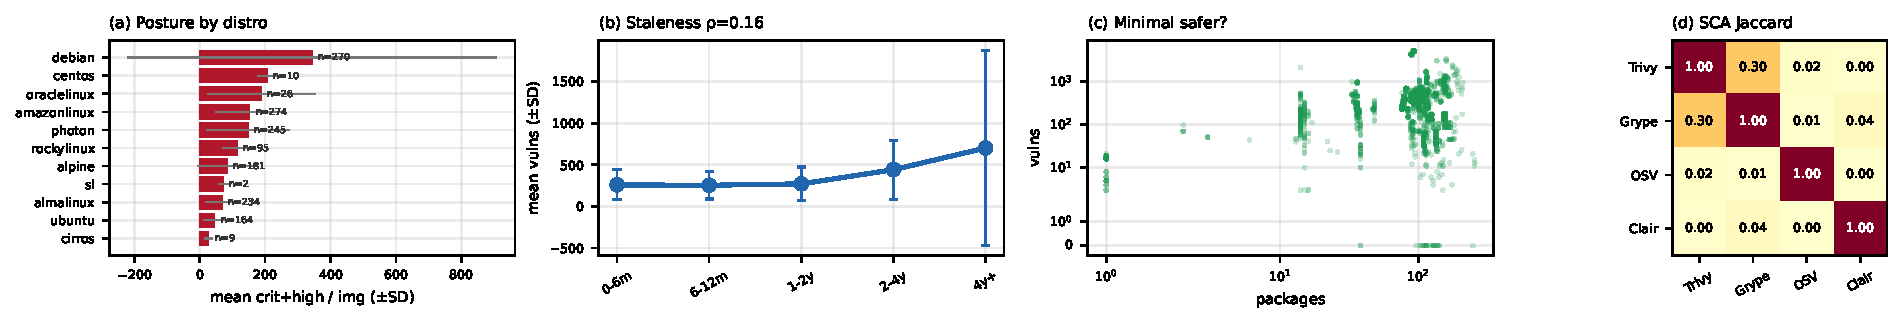
\includegraphics[width=\textwidth]{fig_panels.pdf}
\caption{(a)~mean critical+high vulnerabilities per distribution;
(b)~mean total vulnerabilities by image age; (c)~packages vs.\ vulnerabilities;
(d)~pairwise Jaccard of the four SCA engines over (image, CVE, package).}
\label{fig:panels}
\end{figure}

\subsection{RQ1: Security posture by distribution}
\label{sec:rq1}
Critical- and high-severity vulnerability findings vary by an order of
magnitude across distributions (Figure~\ref{fig:panels}(a)). Debian carries
the most (mean $\approx$344 critical+high per image), followed by the RHEL
family (CentOS $\approx$205, OracleLinux $\approx$189, AmazonLinux $\approx$152,
RockyLinux $\approx$128); Alpine sits much lower ($\approx$84), and Arch, ALT,
Kali and openSUSE~Tumbleweed report essentially none. Package count does not
track this ordering: Mageia and Fedora carry the most packages yet few
critical or high findings, a point we return to in Section~\ref{sec:rq5}.

\subsection{RQ2: Staleness vs.\ vulnerability}
\label{sec:rq2}
Vulnerability count rises monotonically with image age
(Figure~\ref{fig:panels}(b)). Images rebuilt within the last six months carry
a mean of $\approx$255 total vulnerability findings, climbing through
$\approx$273 (one to two years) and $\approx$457 (two to four years) to
$\approx$692 for images not rebuilt in over four years. This reproduces the
technical-lag effect of Zerouali et al.~\cite{zerouali2019outdated} on the
OS-base subset and across 21 distributions at once.

\subsection{RQ3: Inter-scanner divergence on OS packages}
\label{sec:rq3}
The four package-vulnerability engines barely agree (Figure~\ref{fig:panels}).
Over (image, CVE, package) triples the best-agreeing pair is Trivy and Grype, at
a Jaccard of \textbf{0.30}; every other pair is below 0.05, and OSV-Scanner and
Clair are essentially disjoint from the rest (OSV$\cap$Clair $=0$). The engines
differ in scope: Grype and Trivy report the most triples (353k and 227k),
OSV-Scanner targets language-ecosystem advisories (96k), and Clair maps only
specific distributions to its feeds (43k, and zero on Rocky and AlmaLinux,
which it does not map to the RHEL feeds). The reported security posture of an
OS image is thus, to a large degree, a property of the chosen scanner, echoing
Churakova et al.~\cite{churakova2026vex} at far larger scale and on the OS
layer specifically.

\subsection{RQ4: End-of-life and un-pullable images}
\label{sec:rq4}
Two longevity hazards surface. First, about \textbf{20\%} of the digest-pinned
OS images fail to pull on a current Docker Engine with \texttt{manifest schema
unsupported}: they are old images in the deprecated Docker image-manifest
schema~1, whose support modern Docker removed. The digests still exist on
Docker Hub, but the images are no longer installable, a hazard concentrated in
the oldest tags (highest for \texttt{ubuntu}, near zero for \texttt{archlinux}
and \texttt{almalinux}). Second, end-of-life distributions remain in heavy use:
every \texttt{centos} tag has been unmaintained since June~2024, yet the
repository still records over a billion pulls. To our knowledge neither the
prevalence of legacy-schema OS images nor the popularity of EOL bases has been
measured before.

\subsection{RQ5: Is a minimal image safer?}
\label{sec:rq5}
The intuition that a smaller image is a safer one does not hold cleanly
(Figure~\ref{fig:panels}(c)). The relationship between package count and
vulnerability count is not monotonic: BusyBox, with a single package, carries
only a handful of findings, but Mageia, with around 250 packages, carries about
a dozen, while Debian carries hundreds of critical and high findings with fewer
packages than Mageia. This refines Haque and Babar~\cite{haque2022wellbegun}:
on our multi-scanner data the vulnerability count is governed more by a
distribution's advisory coverage and patch cadence than by image size.

\subsection{Reproducing prior analyses}
\label{sec:repro}
Our four questions reproduce, on the OS-base subset specifically, concrete
analyses from prior work (Table~\ref{tab:repro}); the direction holds in every
case, and the multi-scanner setting lets us refine the minimal-image and
scanner-agreement results that single-tool studies could not.

\begin{table}[!htbp]
\centering
\caption{Prior analyses reproduced on our OS-base corpus.}
\label{tab:repro}
\scriptsize
\setlength{\tabcolsep}{3pt}
\renewcommand{\arraystretch}{1.15}
\begin{tabular}{@{}p{0.15\columnwidth} p{0.27\columnwidth} p{0.24\columnwidth} p{0.26\columnwidth}@{}}
\toprule
\textbf{Study} & \textbf{Analysis} & \textbf{Reported there} & \textbf{This corpus} \\
\midrule
Shu et al.~\cite{shu2017dockerhub} & worst-severity prevalence & $>$80\% high-severity & critical/high pervasive; Debian $\approx$344 crit+high per img \\
Zerouali et al.~\cite{zerouali2019outdated} & staleness vs.\ vulns (Debian) & lag grows with age & monotone $\approx$255 to $\approx$692 across 21 distros (RQ2) \\
Haque \& Babar~\cite{haque2022wellbegun} & minimal vs.\ large base & minimal not safer & vulns not monotone in package count (RQ5) \\
Churakova et al.~\cite{churakova2026vex} & scanner agreement, 48 img & Trivy/Grype Jaccard 0.69 & 0.30 over OS images; OSV/Clair disjoint (RQ3) \\
\bottomrule
\end{tabular}
\end{table}

% ============================================================
\section{Conclusion}
\label{sec:conclusion}
We presented a recent, multi-scanner census of the operating-system base images
of Docker Hub, the bases on which nearly every container is built, scanned with
13 independent open-source tools rather than one. Across the images measured so
far, vulnerability posture varies by an order of magnitude across distributions
and rises steadily with image age; the four package-vulnerability engines agree
on almost nothing, so the posture a single tool reports is in large part a
property of that tool; a smaller image is not reliably a safer one; and about a
fifth of historically-published OS images can no longer be installed by a
modern Docker, while end-of-life bases such as CentOS remain heavily pulled. We
release the pipeline and the consolidated dataset\footnote{The scan pipeline,
analysis code and the consolidated multi-scanner dataset will be released on
acceptance.} so the measurement can be reproduced and kept current.

{\footnotesize
\bibliographystyle{sbc}
\bibliography{paper}
}
\end{document}
